\begin{ex}
(Vunesp) Num curso de inglês, a distribuição das idades dos alunos é dada pelo gráfico:
\begin{center}
  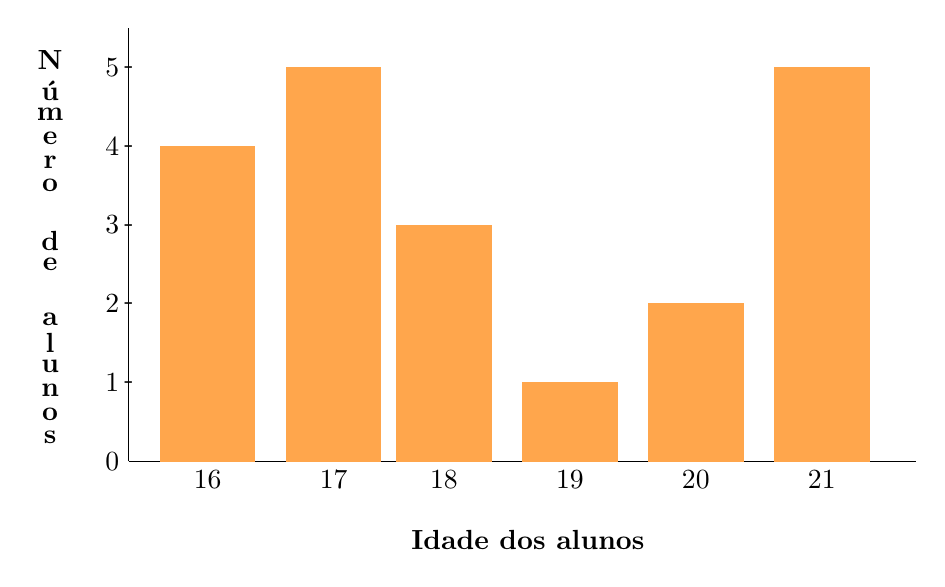
\begin{tikzpicture}
  \draw (0,0)--(10,0); \draw (0,0)--(0,5.5);
  \draw [fill=orange!70, draw=orange!70] (0.4,0) rectangle (1.6,4);
  \draw [fill=orange!70, draw=orange!70] (2,0) rectangle (3.2,5);
  \draw [fill=orange!70, draw=orange!70] (3.4,0) rectangle (4.6,3);
  \draw [fill=orange!70, draw=orange!70] (5,0) rectangle (6.2,1);
  \draw [fill=orange!70, draw=orange!70] (6.6,0) rectangle (7.8,2);
  \draw [fill=orange!70, draw=orange!70] (8.2,0) rectangle (9.4,5);
  \node at (1,0) [below] {16};  \node at (2.6,0) [below] {17};
  \node at (4,0) [below] {18};  \node at (5.6,0) [below] {19};
  \node at (7.2,0) [below] {20}; \node at (8.8,0) [below] {21};
  \node at (5,-1) {\textbf{ Idade dos alunos }};
  \node at (0,1) {-}; \node at (0,1) [left] {1};
  \node at (0,2) {-}; \node at (0,2) [left] {2};
  \node at (0,3) {-}; \node at (0,3) [left] {3};
  \node at (0,4) {-}; \node at (0,4) [left] {4};
  \node at (0,5) {-}; \node at (0,5) [left] {5};
  \node at (0,0) [left] {0};
  \node at (-1,5.1) {\textbf{N}};\node at (-1,4.7) {\textbf{ú}};\node at (-1,4.4) {\textbf{m}};\node at (-1,4.1) {\textbf{e}};\node at (-1,3.8) {\textbf{r}};\node at (-1,3.5) {\textbf{o}};\node at (-1,2.8) {\textbf{d}}; \node at (-1,2.5) {\textbf{e}};\node at (-1,1.8) {\textbf{a}};\node at (-1,1.5) {\textbf{l}};\node at (-1,1.2) {\textbf{u}};\node at (-1,.9) {\textbf{n}};\node at (-1,.6) {\textbf{o}};\node at (-1,.3) {\textbf{s}};
   \end{tikzpicture}
\end{center}
Com base nesses dados, determine:
   \begin{enumerate}[(a)]
   \item o número total de alunos do curso e o número de alunos com no mínimo 19 anos.
   \item escolhido um aluno ao acaso, qual a probabilidade de sua idade ser no mínimo 19 anos ou ser exatamente 16 anos.
   \end{enumerate}
     \begin{sol}
      \phantom{A}
      \begin{enumerate} [(a)]
          \item $4+5+3+1+2+5=20$ \\
          no mínimo 19 anos $\rightarrow 1+2+5=8$
          \item $\frac{8}{20}+\frac{4}{20}=\frac{12}{20}=\frac{3}{5}$
      \end{enumerate}
     \end{sol}
\end{ex}